\documentclass[titlepage, 12pt, oneside]{article}

\usepackage[dvipsnames,table]{xcolor} 

\definecolor{Gray}{gray}{0.5}

\usepackage{float}

\usepackage{hyphenat}

\usepackage{setspace}

\linespread{1.5}

\usepackage[english]{babel}

\usepackage{chngcntr}
\counterwithin{figure}{section}
\counterwithin{table}{section}

\usepackage{mathtools}
\usepackage{amsmath}
\numberwithin{equation}{section}

\usepackage{caption}

\usepackage[T1]{fontenc}

\usepackage{lmodern}

\usepackage{newtxtext,newtxmath}

\usepackage{listings}

\usepackage[numbered]{matlab-prettifier}

\lstset{style=Matlab-editor,
	basicstyle=\mlttfamily,
	breaklines=true,
	breakindent=0pt}

\usepackage{enumerate}

\usepackage{enumitem}

\usepackage{etoolbox}
\AtBeginEnvironment{thebibliography}{\setlength{\leftskip}{0pt}\setlength{\itemindent}{0pt}}

\setlist[itemize]{leftmargin=*}

\usepackage{graphicx}
\graphicspath{{figures/}}

\usepackage[a4paper, top=2.5cm, bottom=2.5cm, left=3cm, right=2.5cm]{geometry}

\usepackage{fancyhdr, ifthen}
\pagestyle{fancy}
\fancyhf{}
\lhead{South African Crime Statistics Analysis}
\rhead{Page \thepage}

\renewcommand{\headrulewidth}{0.5pt}
\renewcommand{\footrulewidth}{0.5pt}

\fancyheadoffset[R]{0pt}

\usepackage{xurl}

\usepackage[breaklinks,linktocpage=true]{hyperref}

\hypersetup{colorlinks=true,urlcolor=blue,linkcolor=blue,citecolor=blue}
\urlstyle{same}

\usepackage{multirow}

\usepackage{booktabs}

\usepackage{array}

\usepackage{eso-pic}

\usepackage{subcaption}

\usepackage{appendix}

\usepackage{adjustbox}

\usepackage{pdflscape}

\usepackage[most]{tcolorbox}

\usepackage{tabularx}
\newcolumntype{Y}{>{\centering\arraybackslash}X}

\makeatletter
\AtBeginDocument{\renewcommand{\bibname}{References}}
\renewcommand\@biblabel[1]{}
\renewenvironment{thebibliography}[1]
{\phantomsection\section*{\refname}%
	\@mkboth{\MakeUppercase\refname}{\MakeUppercase\refname}%
	\renewcommand{\bibname}{References}
	\list{}%
	{\leftmargin0pt
		\itemindent0pt
		\labelwidth0pt
		\labelsep0pt
		\@openbib@code
		\usecounter{enumiv}}%
	\sloppy
	\clubpenalty4000
	\@clubpenalty \clubpenalty
	\widowpenalty4000%
	\sfcode`\.\@m}
{\def\@noitemerr
	{\@latex@warning{Empty `thebibliography' environment}}%
	\endlist}
\makeatother

\usepackage[nottoc]{tocbibind}

\usepackage[titles]{tocloft}

\setlength{\cftfigindent}{0pt}

\usepackage{titlesec}

\titleformat{\subsection}
{\normalfont\large\bfseries\color[HTML]{2E7D32}}
{\thesubsection}{1em}{}

\AtBeginDocument{\renewcommand\contentsname {Contents}}

\usepackage{microtype}

\makeatletter
\def\l@lstlisting#1#2{\@dottedtocline{1}{2pt}{0pt}{#1}{#2}}
\makeatother

\hypersetup{pdfstartview={XYZ null null null}}

\usepackage[noadjust]{cite}
\renewcommand*{\citeleft}{}
\renewcommand*{\citeright}{}
\newcommand*{\citename}[1]{#1}

\begin{document}
	
	\begin{titlepage}
		\centering
		
		% top green bar
		\textcolor[HTML]{2E7D32}{\rule{\linewidth}{4pt}}
		
		\vspace{1.5cm}
		
		{\Large \textbf{Data Science Career Portfolio}}
		
		\vspace{1.2cm}
		
		\textcolor[HTML]{2E7D32}{\rule{0.8\linewidth}{1pt}}
		
		\vspace{0.5cm}
		
		{\Huge \textbf{Exploring South African\\[0.3cm] Crime Trends}}
		
		\vspace{0.4cm}
		
		{\Large \textbf{\textcolor[HTML]{2E7D32}{A Data-Driven Analysis (2011--2022)}}}
		
		\vspace{0.5cm}
		
		{\large An Exploratory Data Analysis Report}
		
		\vspace{0.4cm}
		
		{\large SAPS Annual Crime Statistics $\bullet$ Kaggle}
		
		\vspace{0.5cm}
		
		% horizontal rule
		\textcolor[HTML]{2E7D32}{\rule{0.8\linewidth}{1pt}}
		
		\vspace{1.2cm}
		
		{\large Prepared by}
		
		\vspace{0.3cm}
		
		{\Large \textbf{Joshua Pillay}}
		
		\vspace{0.8cm}
		
		{\large \textcolor[HTML]{2E7D32}{\textbf{Tools Used:}}}\\[0.03cm] 
		{\large Excel $\bullet$ SQL $\bullet$ Python $\bullet$ MATLAB $\bullet$ Power BI $\bullet$ R (Appendix)}
		
		\vspace{0.5cm}
		
		{\large \textcolor[HTML]{2E7D32}{\textbf{Repository:}}}\\[0.03cm] 
		{\large \url{github.com/username/sa-crime-statistics}}
		
		\vspace{0.6cm}
		
		{\large May 2026}
		
		\vspace{\fill}
		
		% bottom green bar
		\textcolor[HTML]{2E7D32}{\rule{\linewidth}{4pt}}
		
	\end{titlepage}
	
	% ── FRONT MATTER ──────────────────────────────────────────────
	
	\pagenumbering{roman}
	
	% Abstract
	\newpage
	\section*{Abstract}
	\addcontentsline{toc}{section}{Abstract}
	
	% placeholder — write last
	\newpage
	
	% Table of Contents
	\tableofcontents
	
	\newpage
	
	% List of Figures
	\listoffigures
	
	\newpage
	
	% ── REPORT BODY ───────────────────────────────────────────────
	
	\pagenumbering{arabic}
	
	% ── SECTION 1 ─────────────────────────────────────────────────
	
	\newpage
	\section{Introduction}
	
	\subsection{Background and Context}
	
	\subsection{Research Questions}
	
	\begin{itemize}
		\item \textbf{RQ1:} Which provinces have the highest overall crime rates, and how do they compare to one another?
		\item \textbf{RQ2:} Which crime categories are most prevalent, and have they been increasing or decreasing over time?
		\item \textbf{RQ3:} Are there identifiable seasonal or cyclical patterns in national crime data across the 12-year window?
		\item \textbf{RQ4:} Can a reasonable short-term forecast be produced for a selected crime category?
	\end{itemize}
	
	\subsection{Report Structure}
	
	% ── SECTION 2 ─────────────────────────────────────────────────
	
	\newpage
	\section{Data \& Methodology}
	
	\subsection{Dataset Description}
	
	\begin{table}[H]
		\centering
		\caption{Dataset variable descriptions}
		\begin{tabularx}{\linewidth}{llX}
			\toprule
			\textbf{Variable} & \textbf{Type} & \textbf{Description} \\
			\midrule
			\texttt{province}        & Dimension & One of South Africa's nine provinces. Renamed from \texttt{Geography} during cleaning. \\[0.3cm]
			\texttt{crime\_category} & Dimension & Broad crime category — seven categories, renamed to shorter chart-friendly versions during cleaning. \\[0.3cm]
			\texttt{financial\_year} & Dimension & Start year of the financial year, parsed from text to integer (2011–2022). \\[0.3cm]
			\texttt{incident\_count} & Measure   & Number of reported crime incidents for that province, category, and year. \\
			\bottomrule
		\end{tabularx}
	\end{table}
	
	\subsection{Data Quality}
	
	\subsection{Analytical Pipeline}
	
	% ── SECTION 3 ─────────────────────────────────────────────────
	
	\newpage
	\section{Exploratory Analysis}
	
	\subsection{Provincial Crime Distribution (RQ1)}
	
	\begin{figure}[H]
		\centering
		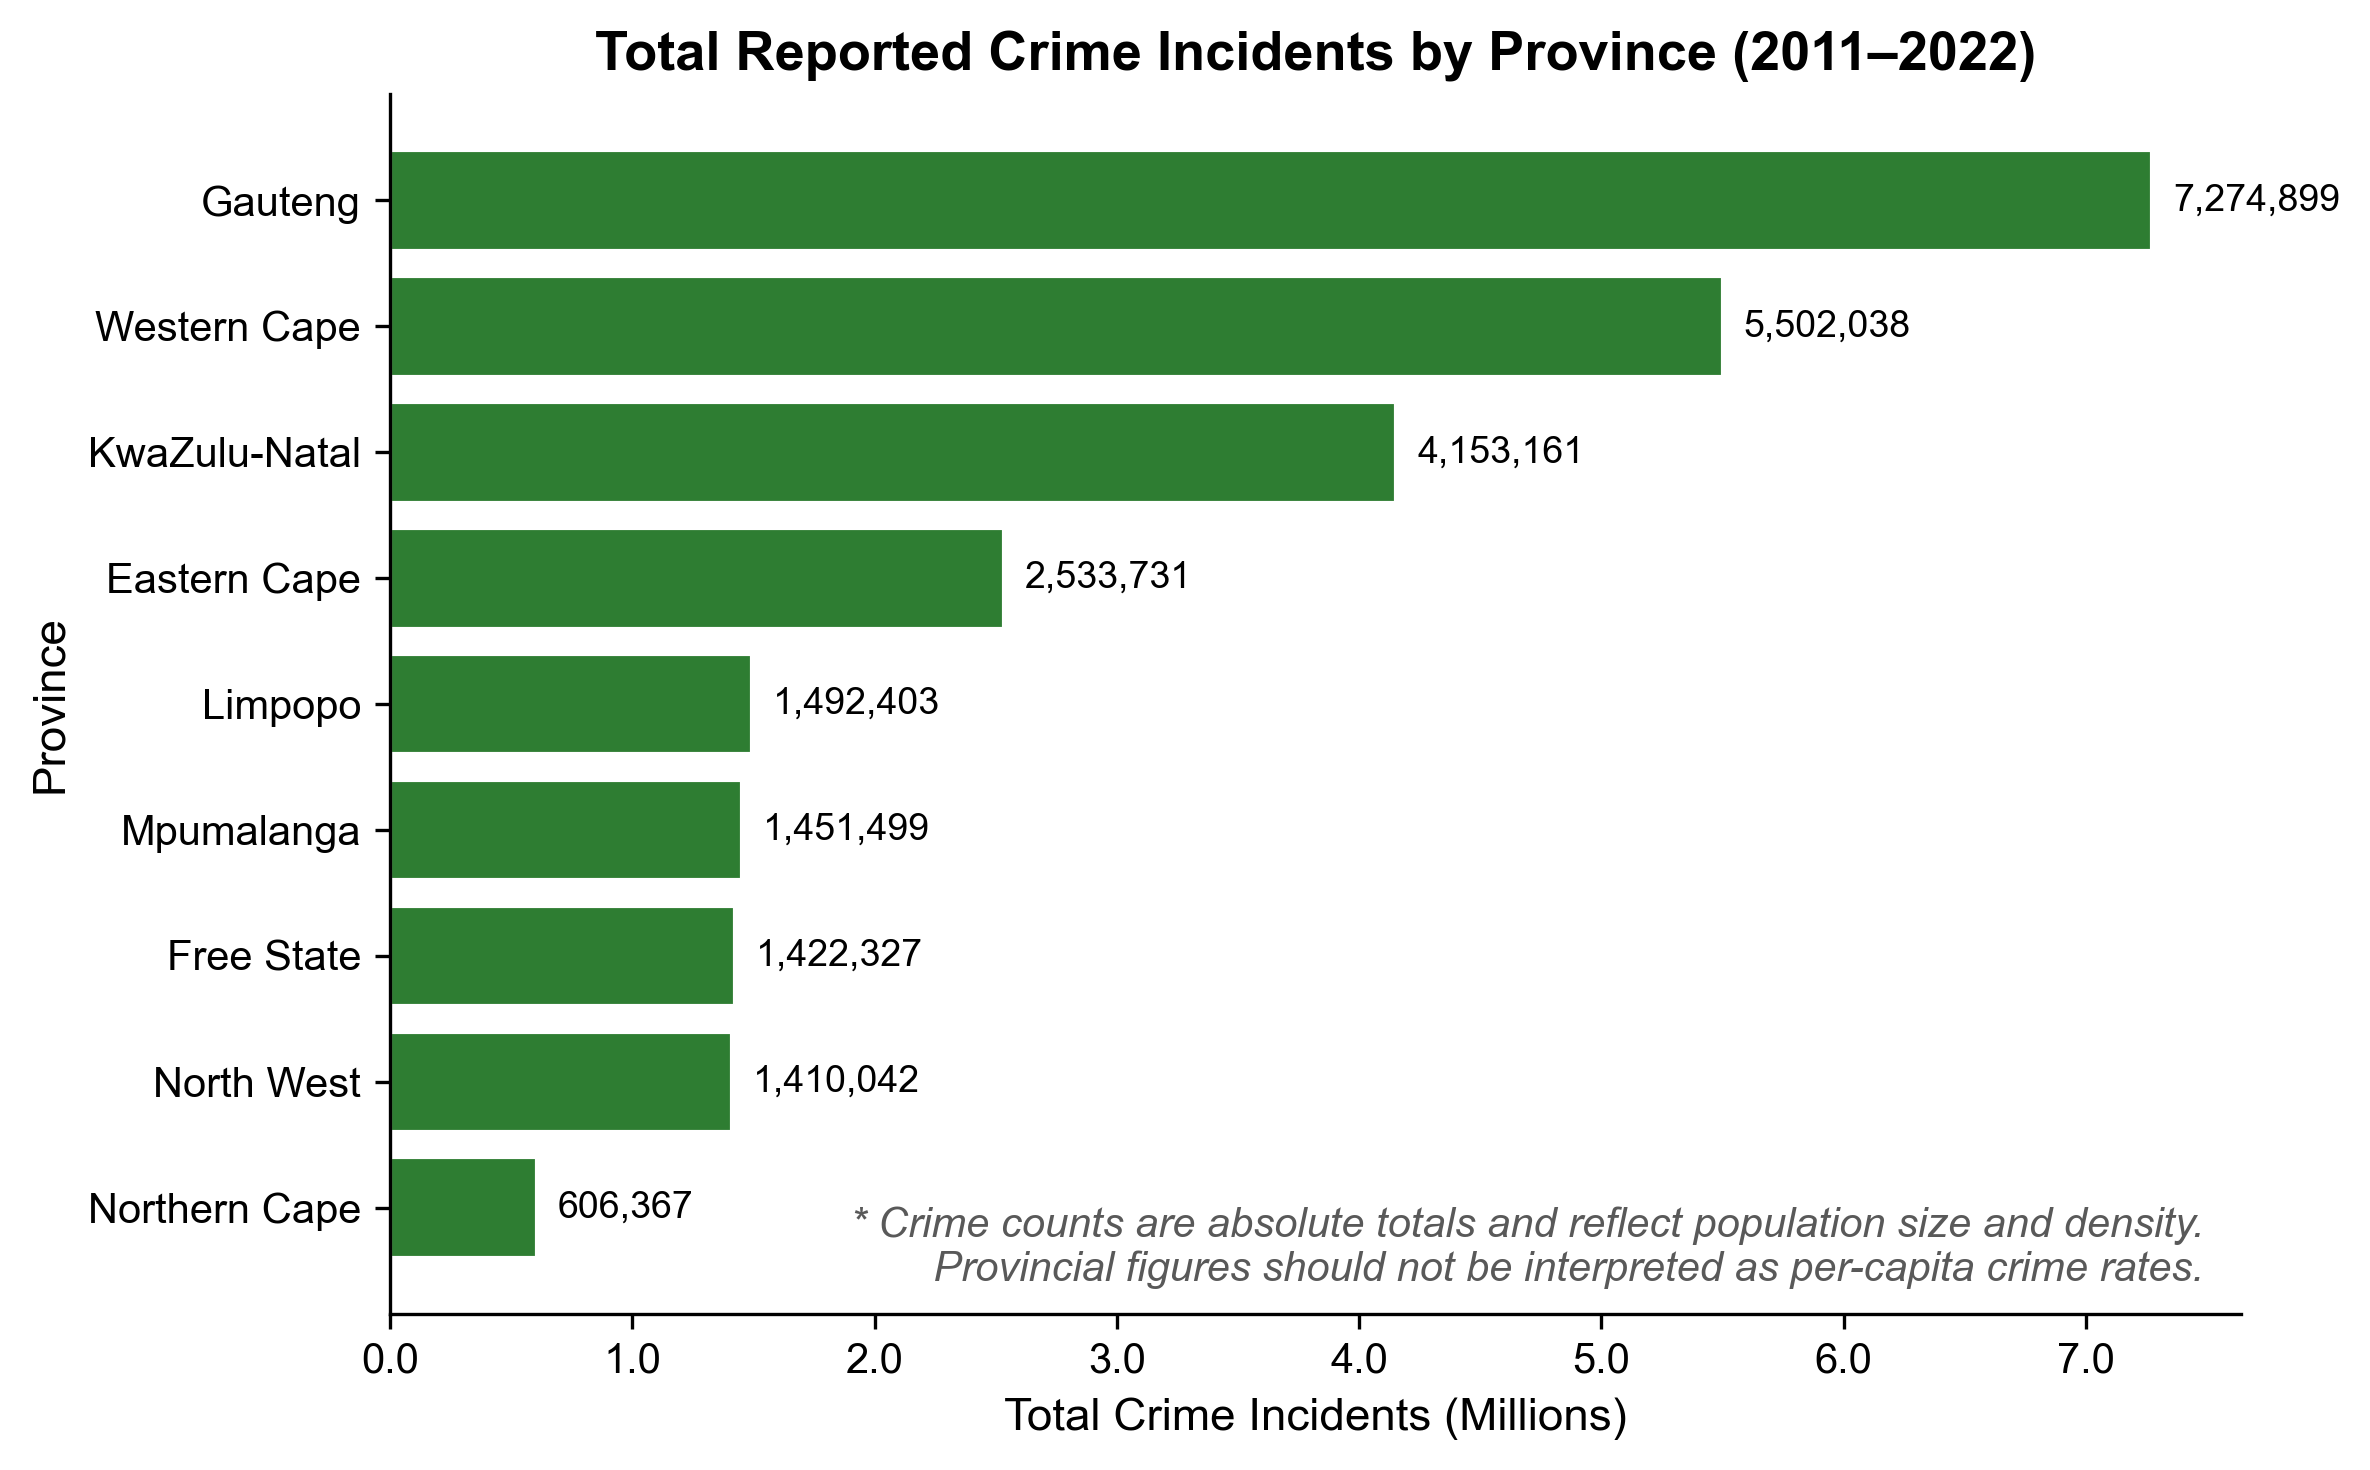
\includegraphics[width=\linewidth]{province_bar_chart.png}
		\caption{Total reported crimes by province, 2011--2022 (Python — matplotlib)}
		\label{fig:province_bar}
	\end{figure}
	
	\subsubsection{SQL Cross-Validation}
	
	\subsection{Crime Category Trends (RQ2)}
	
	\begin{figure}[H]
		\centering
		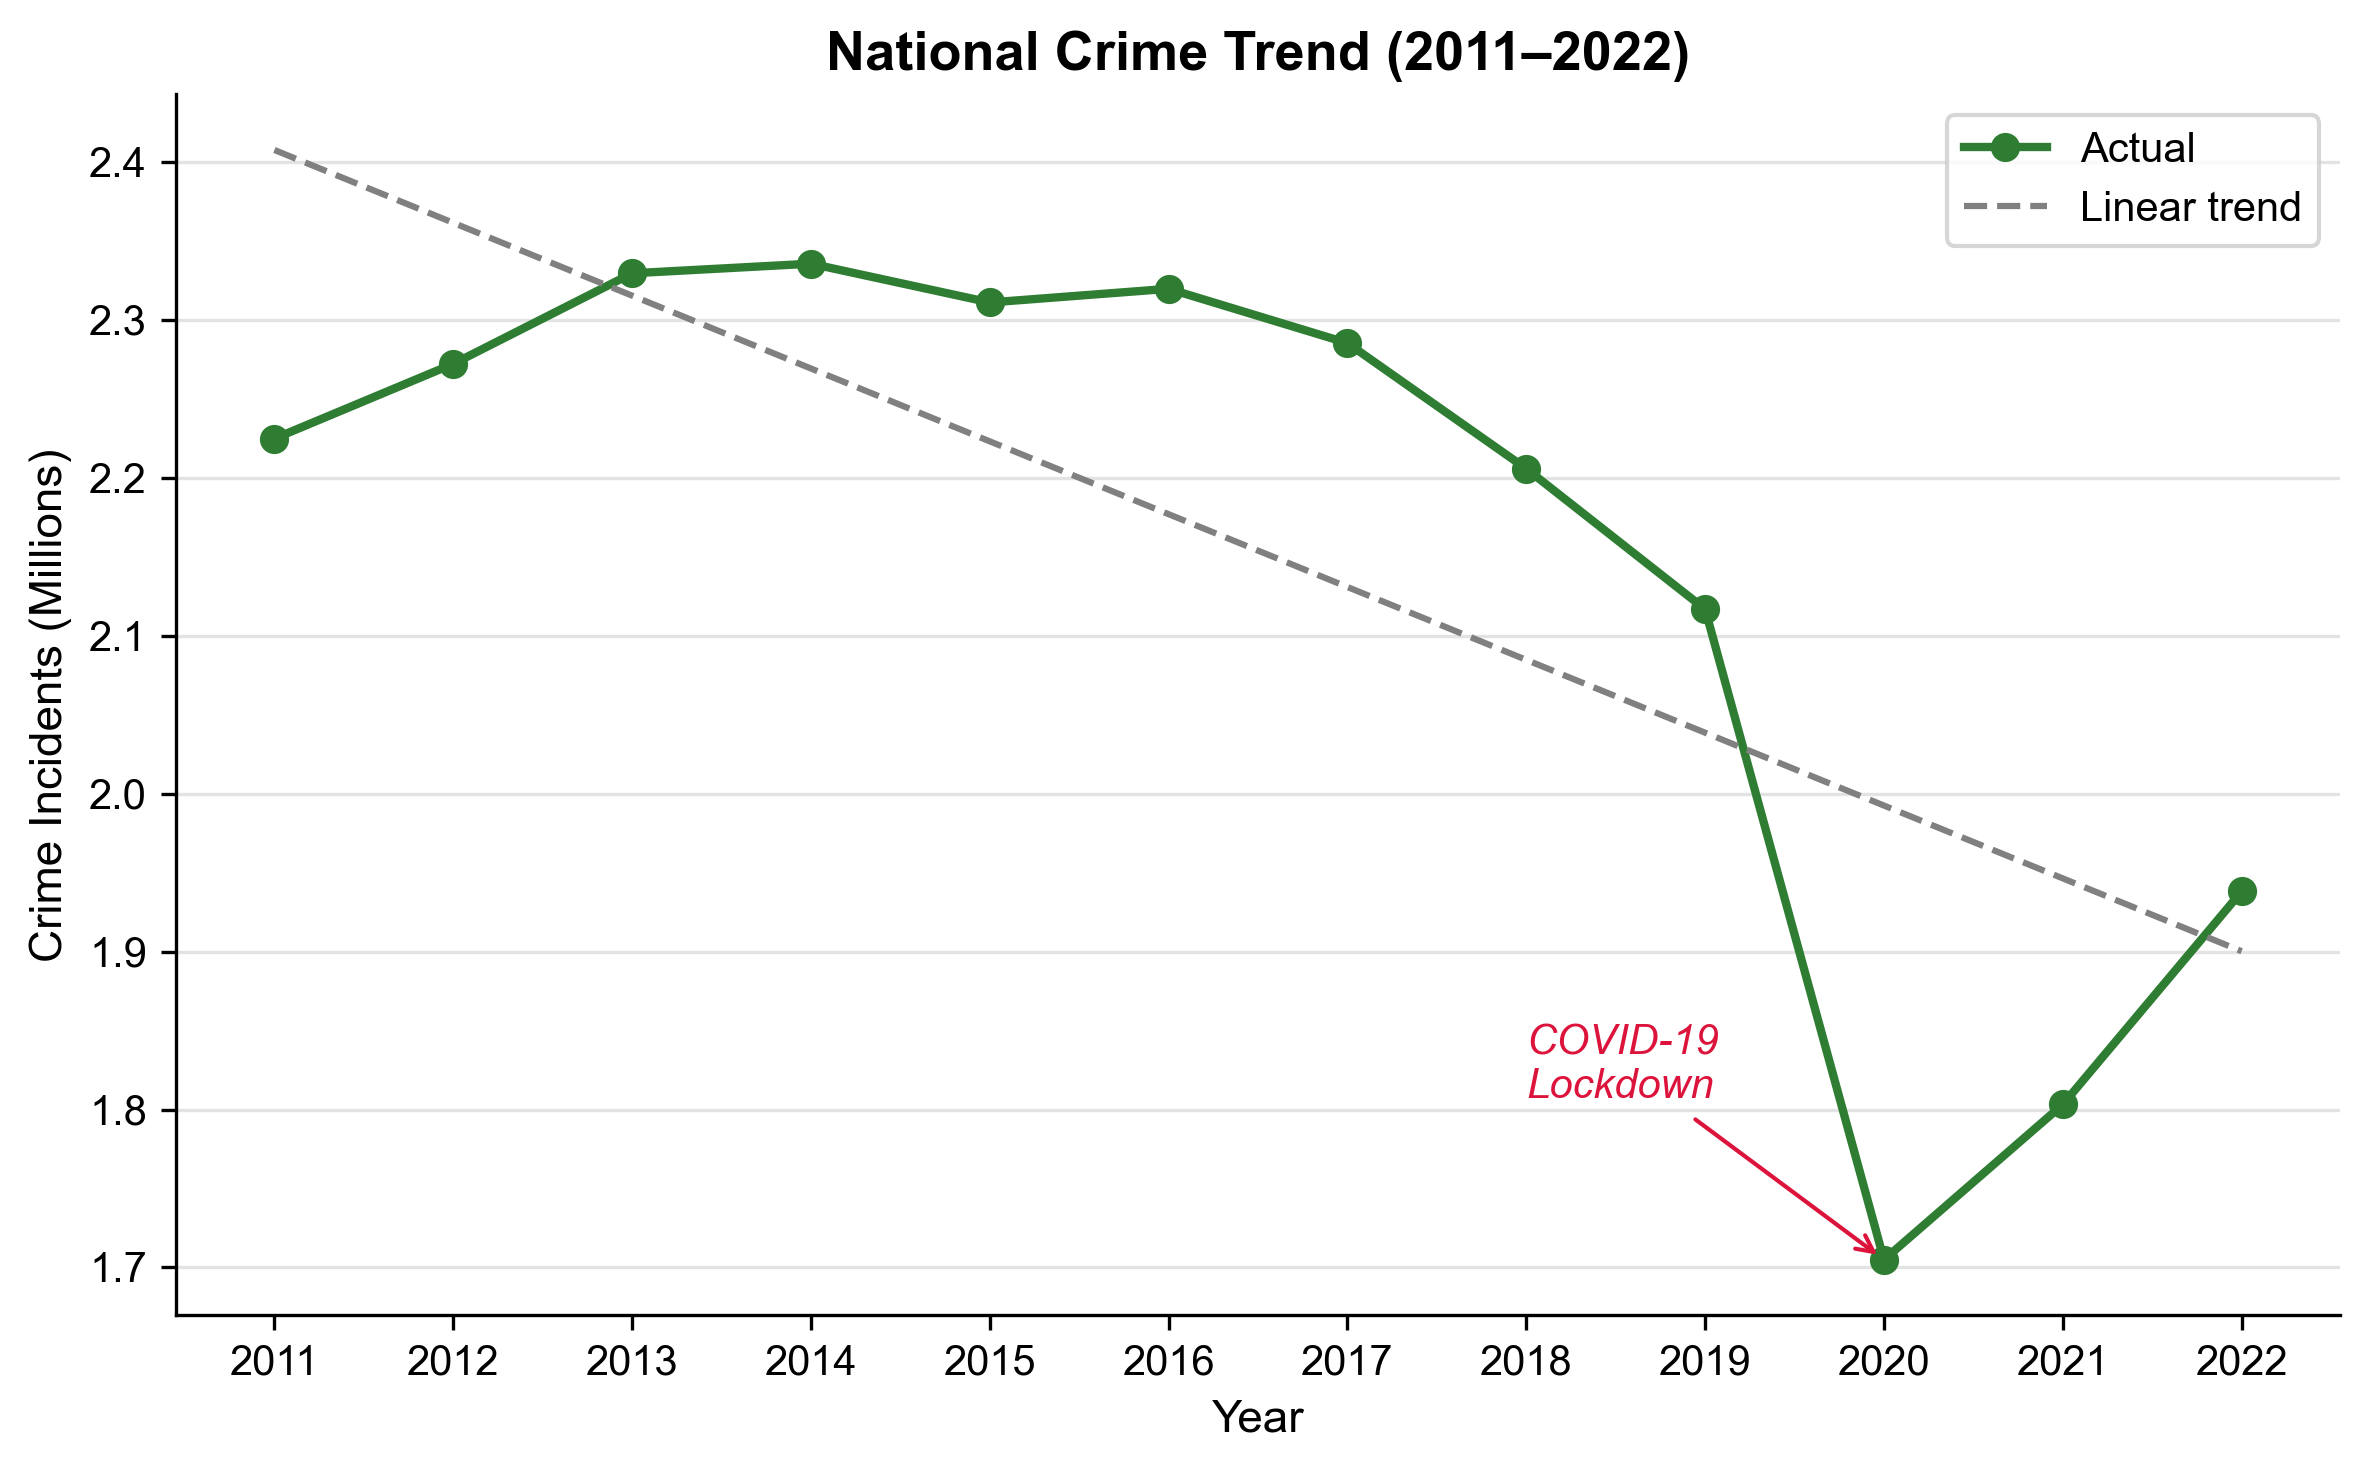
\includegraphics[width=\linewidth]{national_crime_trend.png}
		\caption{National crime trend with COVID-19 annotation (Python — matplotlib)}
		\label{fig:national_trend}
	\end{figure}
	
	\begin{figure}[H]
		\centering
		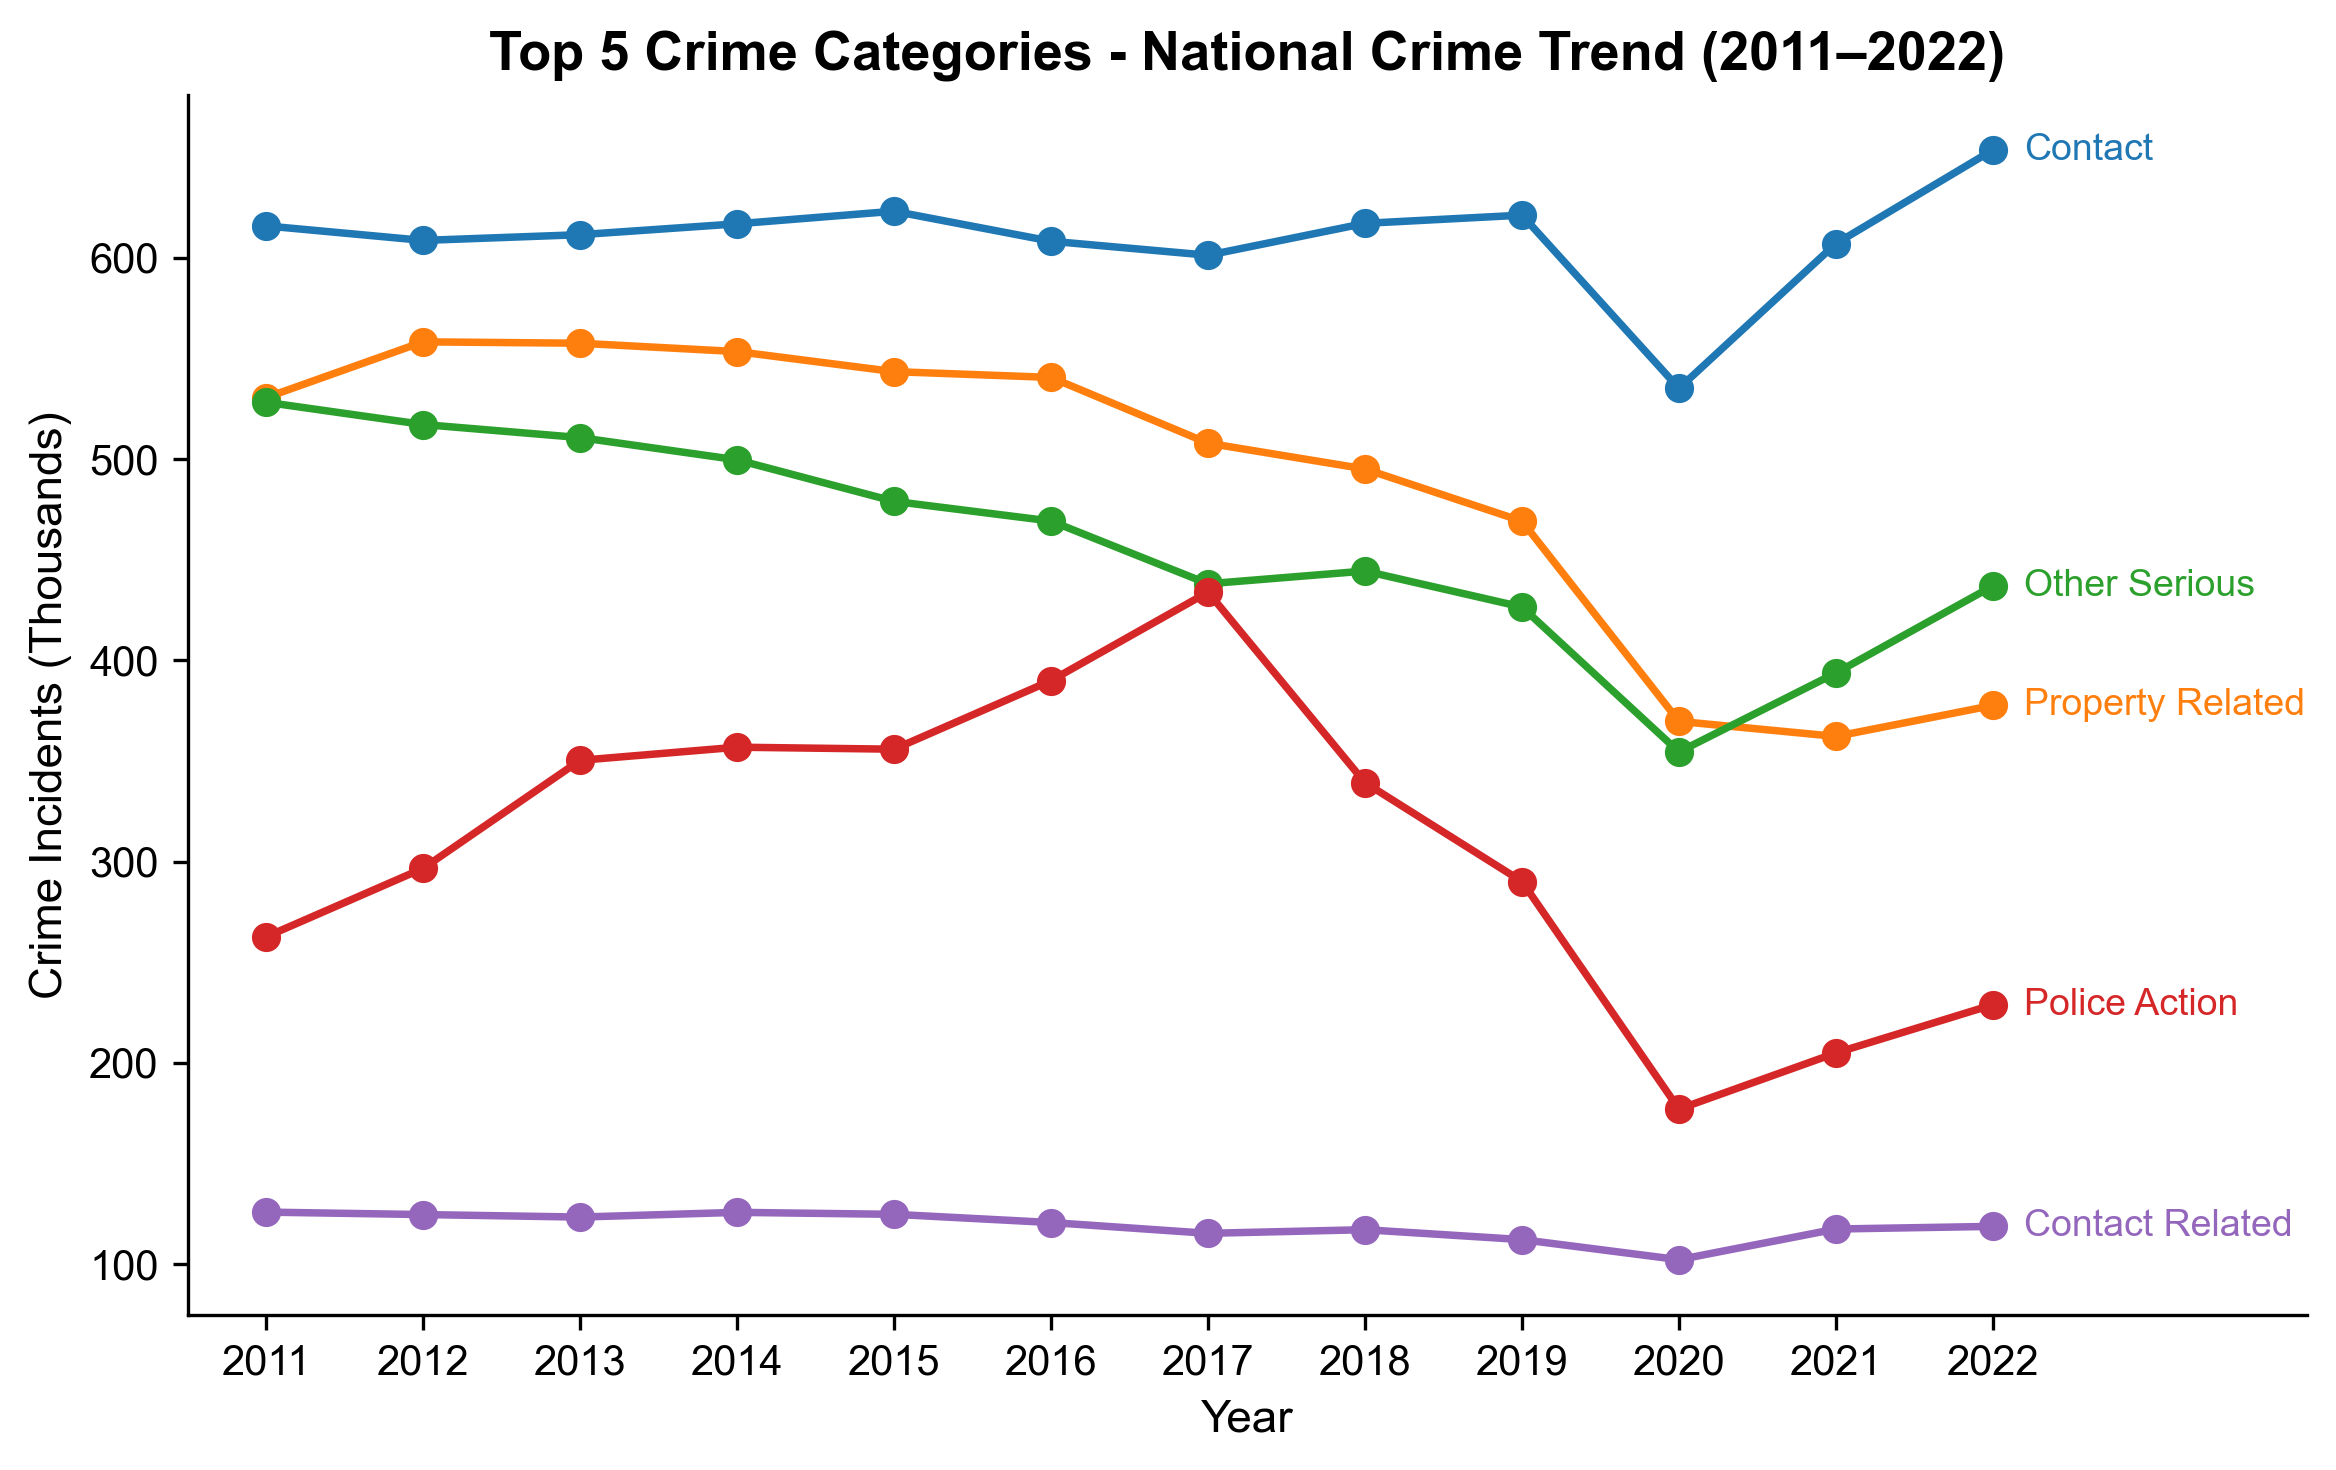
\includegraphics[width=\linewidth]{top5_categories.png}
		\caption{Top 5 crime categories: national trend 2011--2022 (Python — matplotlib)}
		\label{fig:top5}
	\end{figure}
	
	\begin{landscape}
		\thispagestyle{empty}
		\begin{figure}[H]
			\centering
			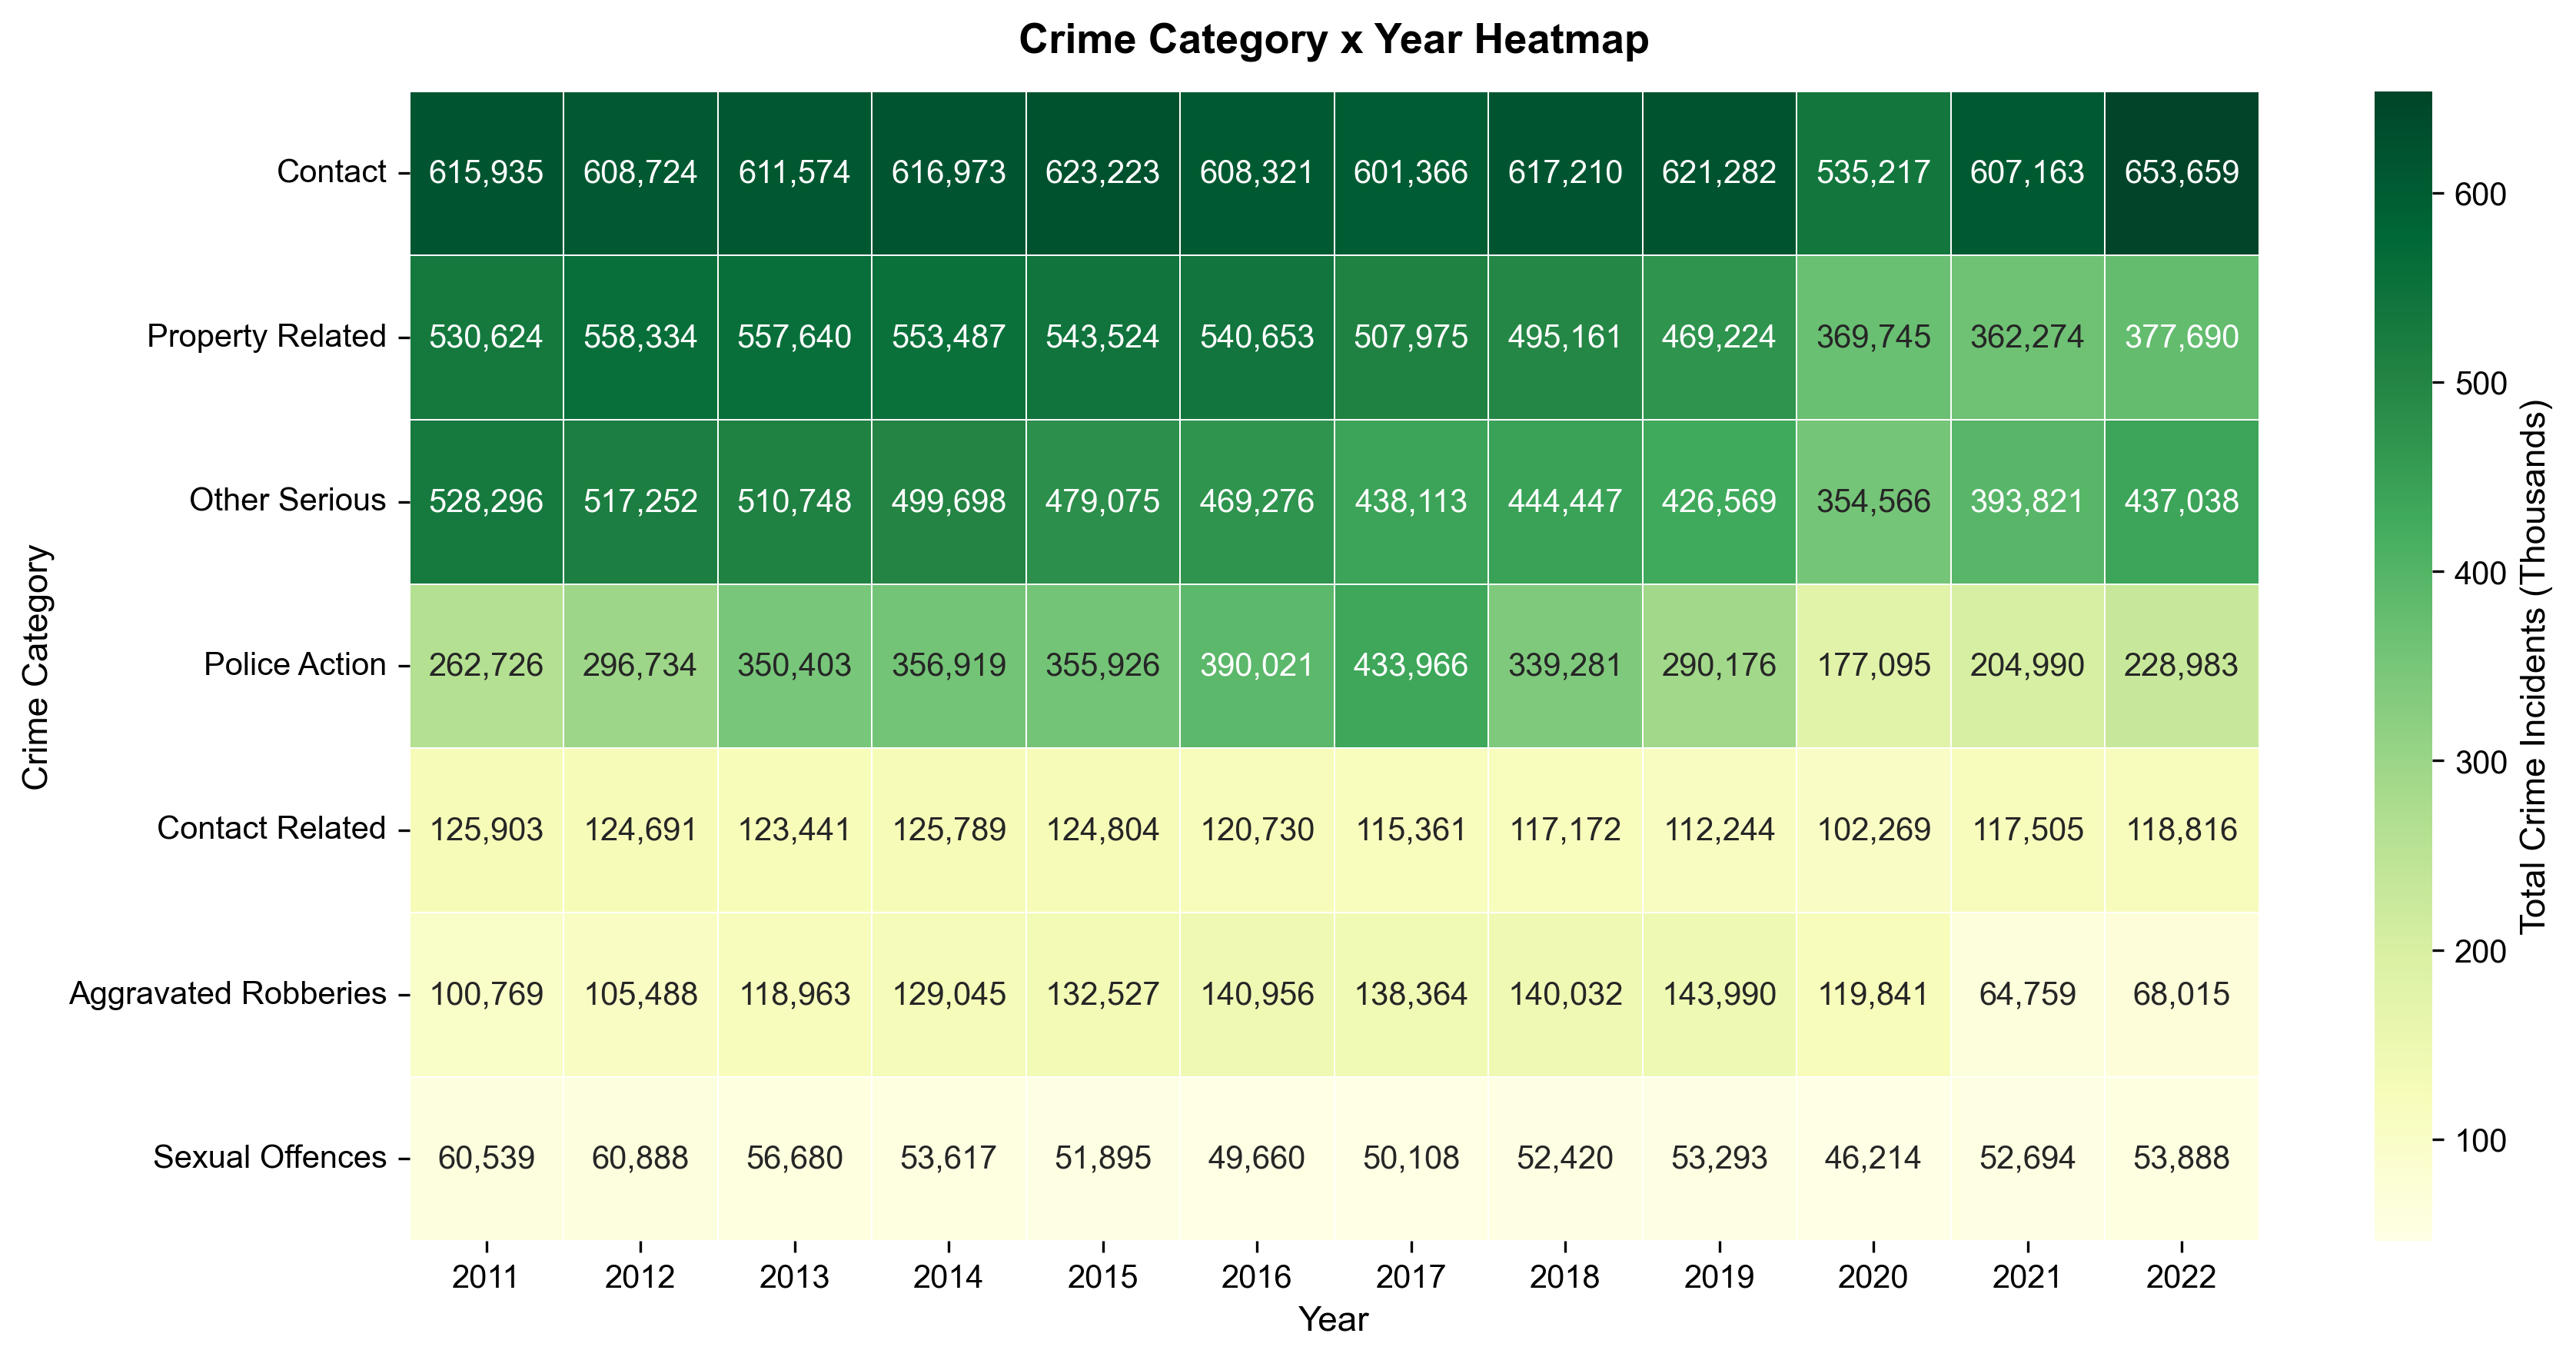
\includegraphics[width=\linewidth]{category_year_heatmap.png}
			\caption{Crime category $\times$ year heatmap, total count (Python — matplotlib, YlGn)}
			\label{fig:heatmap}
		\end{figure}
	\end{landscape}
	
	\subsubsection{SQL Cross-Validation}
	
	\subsection{Seasonal and Cyclical Patterns (RQ3)}
	
	\subsection{Geospatial Analysis (RQ1)}
	
	\begin{figure}[H]
		\centering
		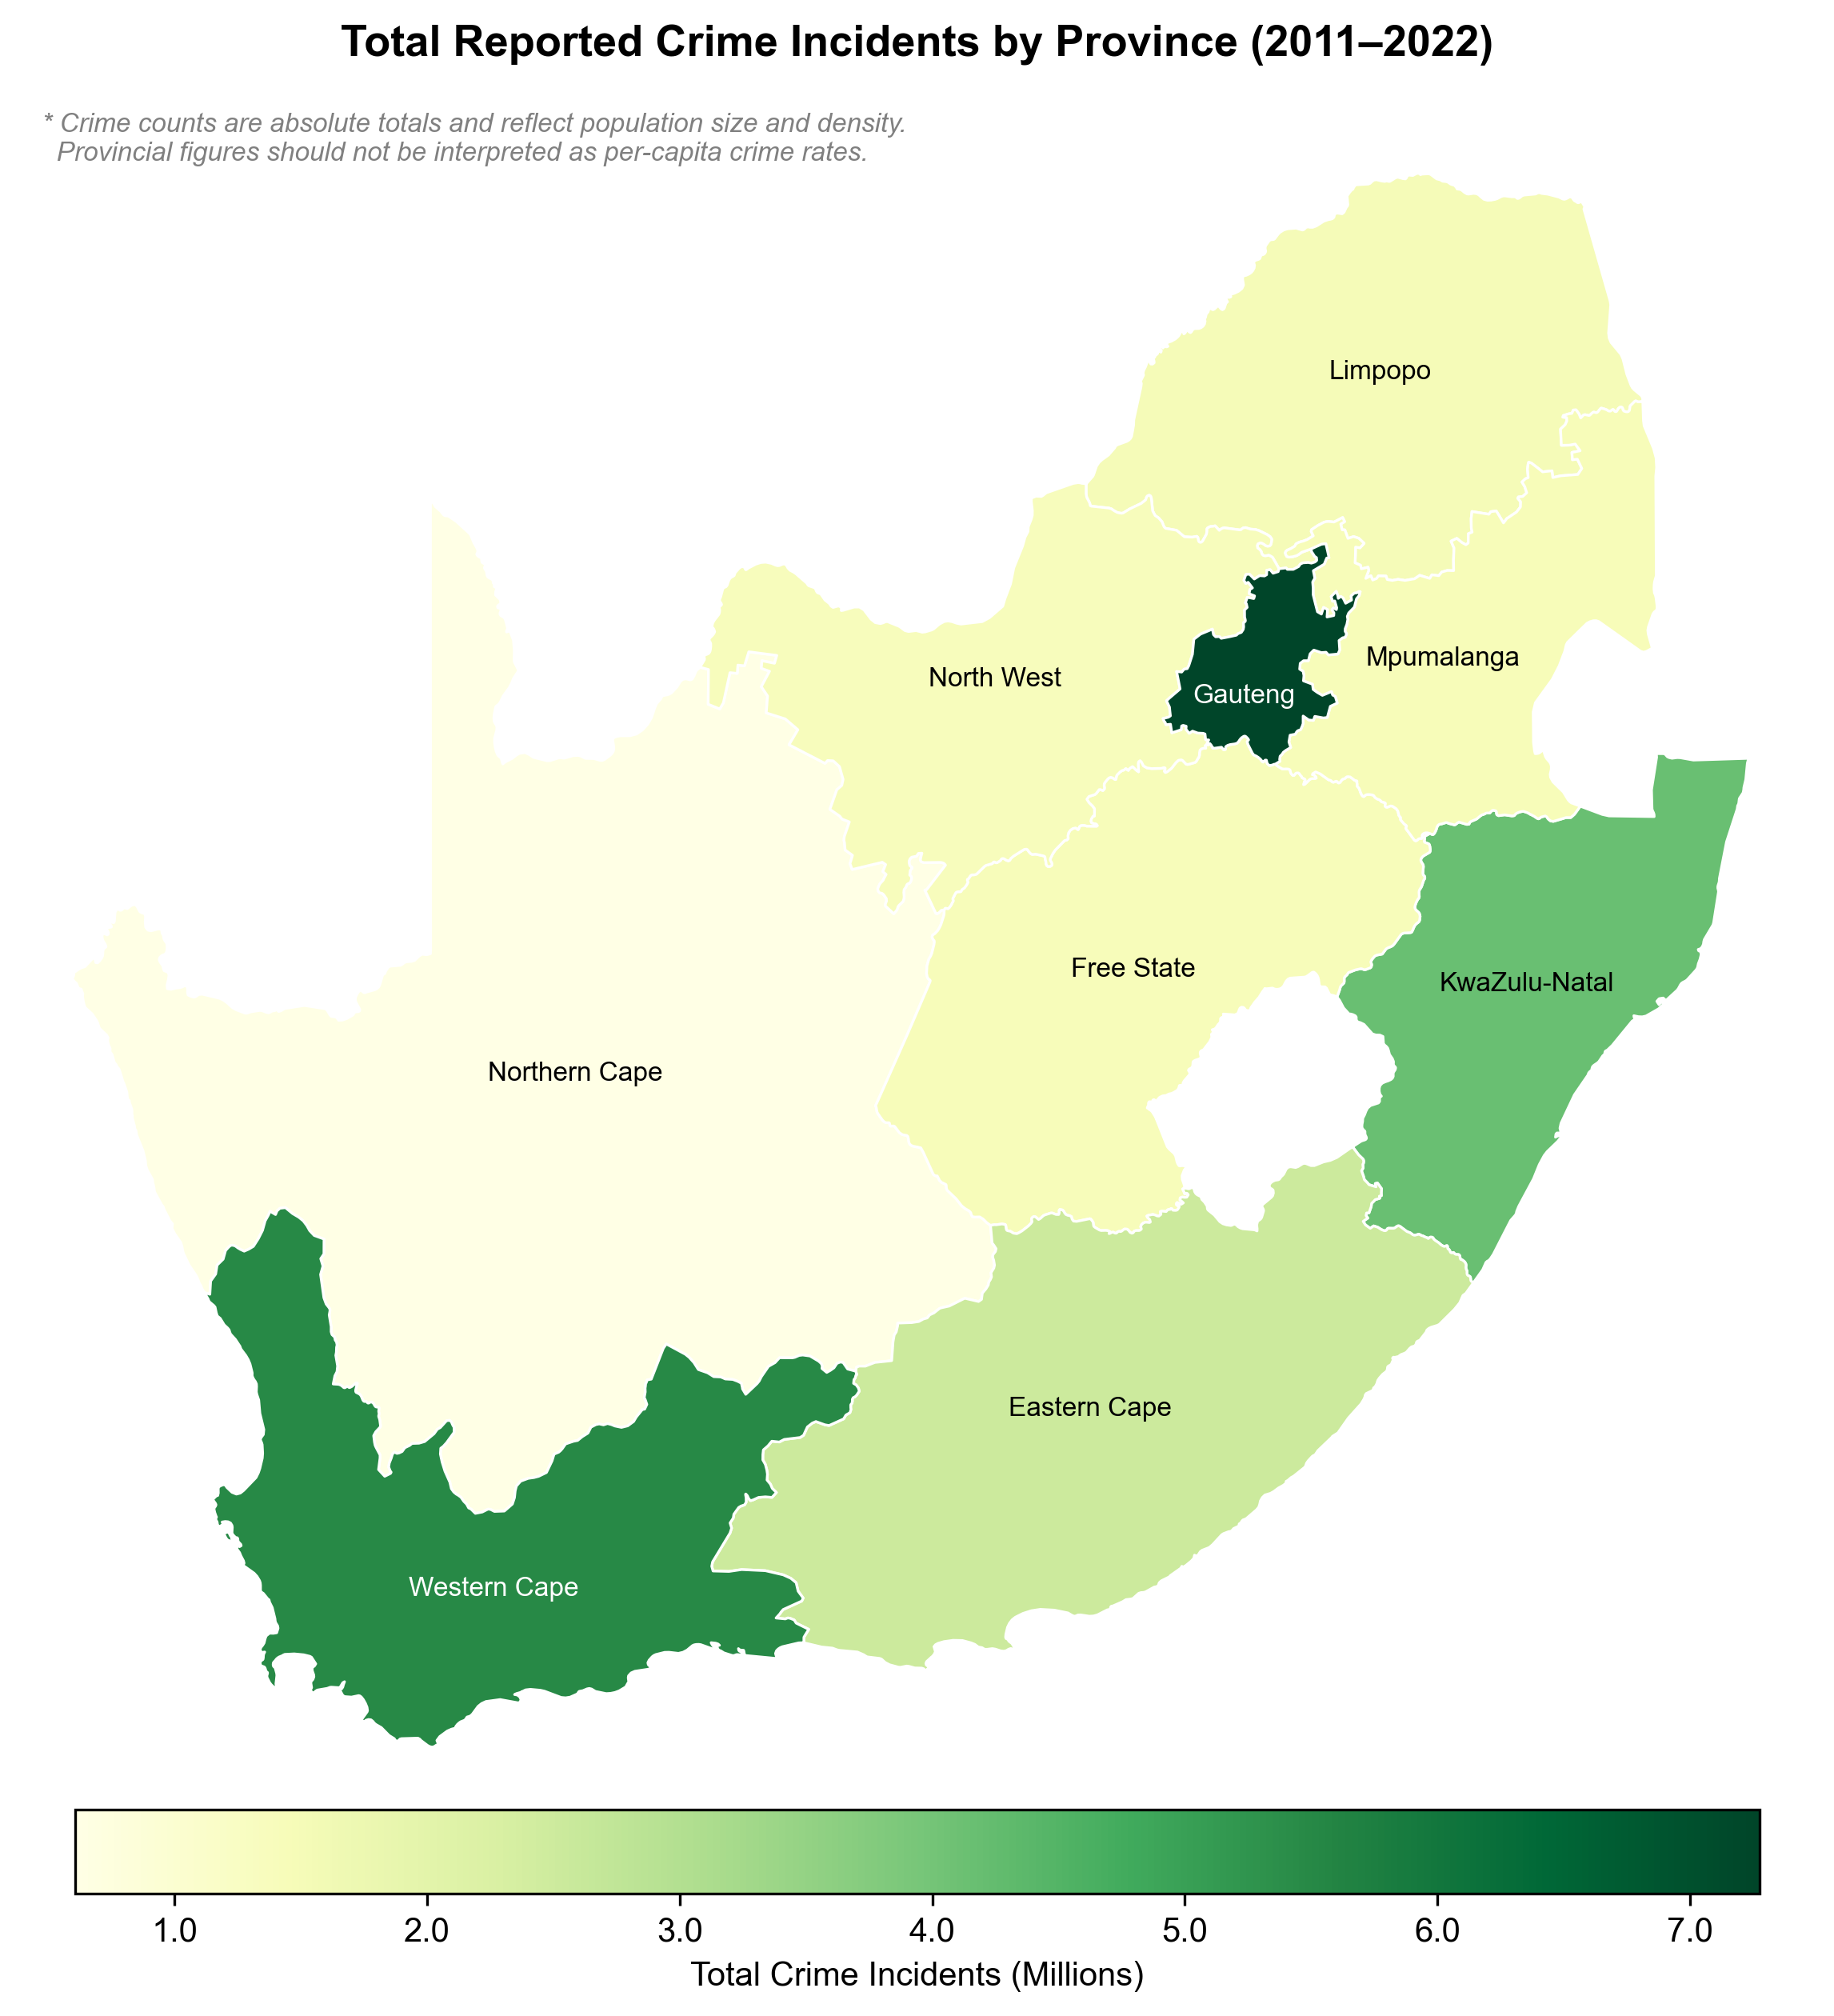
\includegraphics[width=\linewidth]{choropleth_total.png}
		\caption{Choropleth map — total crime incidents by province, all years (Python — geopandas, matplotlib)}
		\label{fig:choropleth_total}
	\end{figure}
	
	\begin{figure}[H]
		\centering
		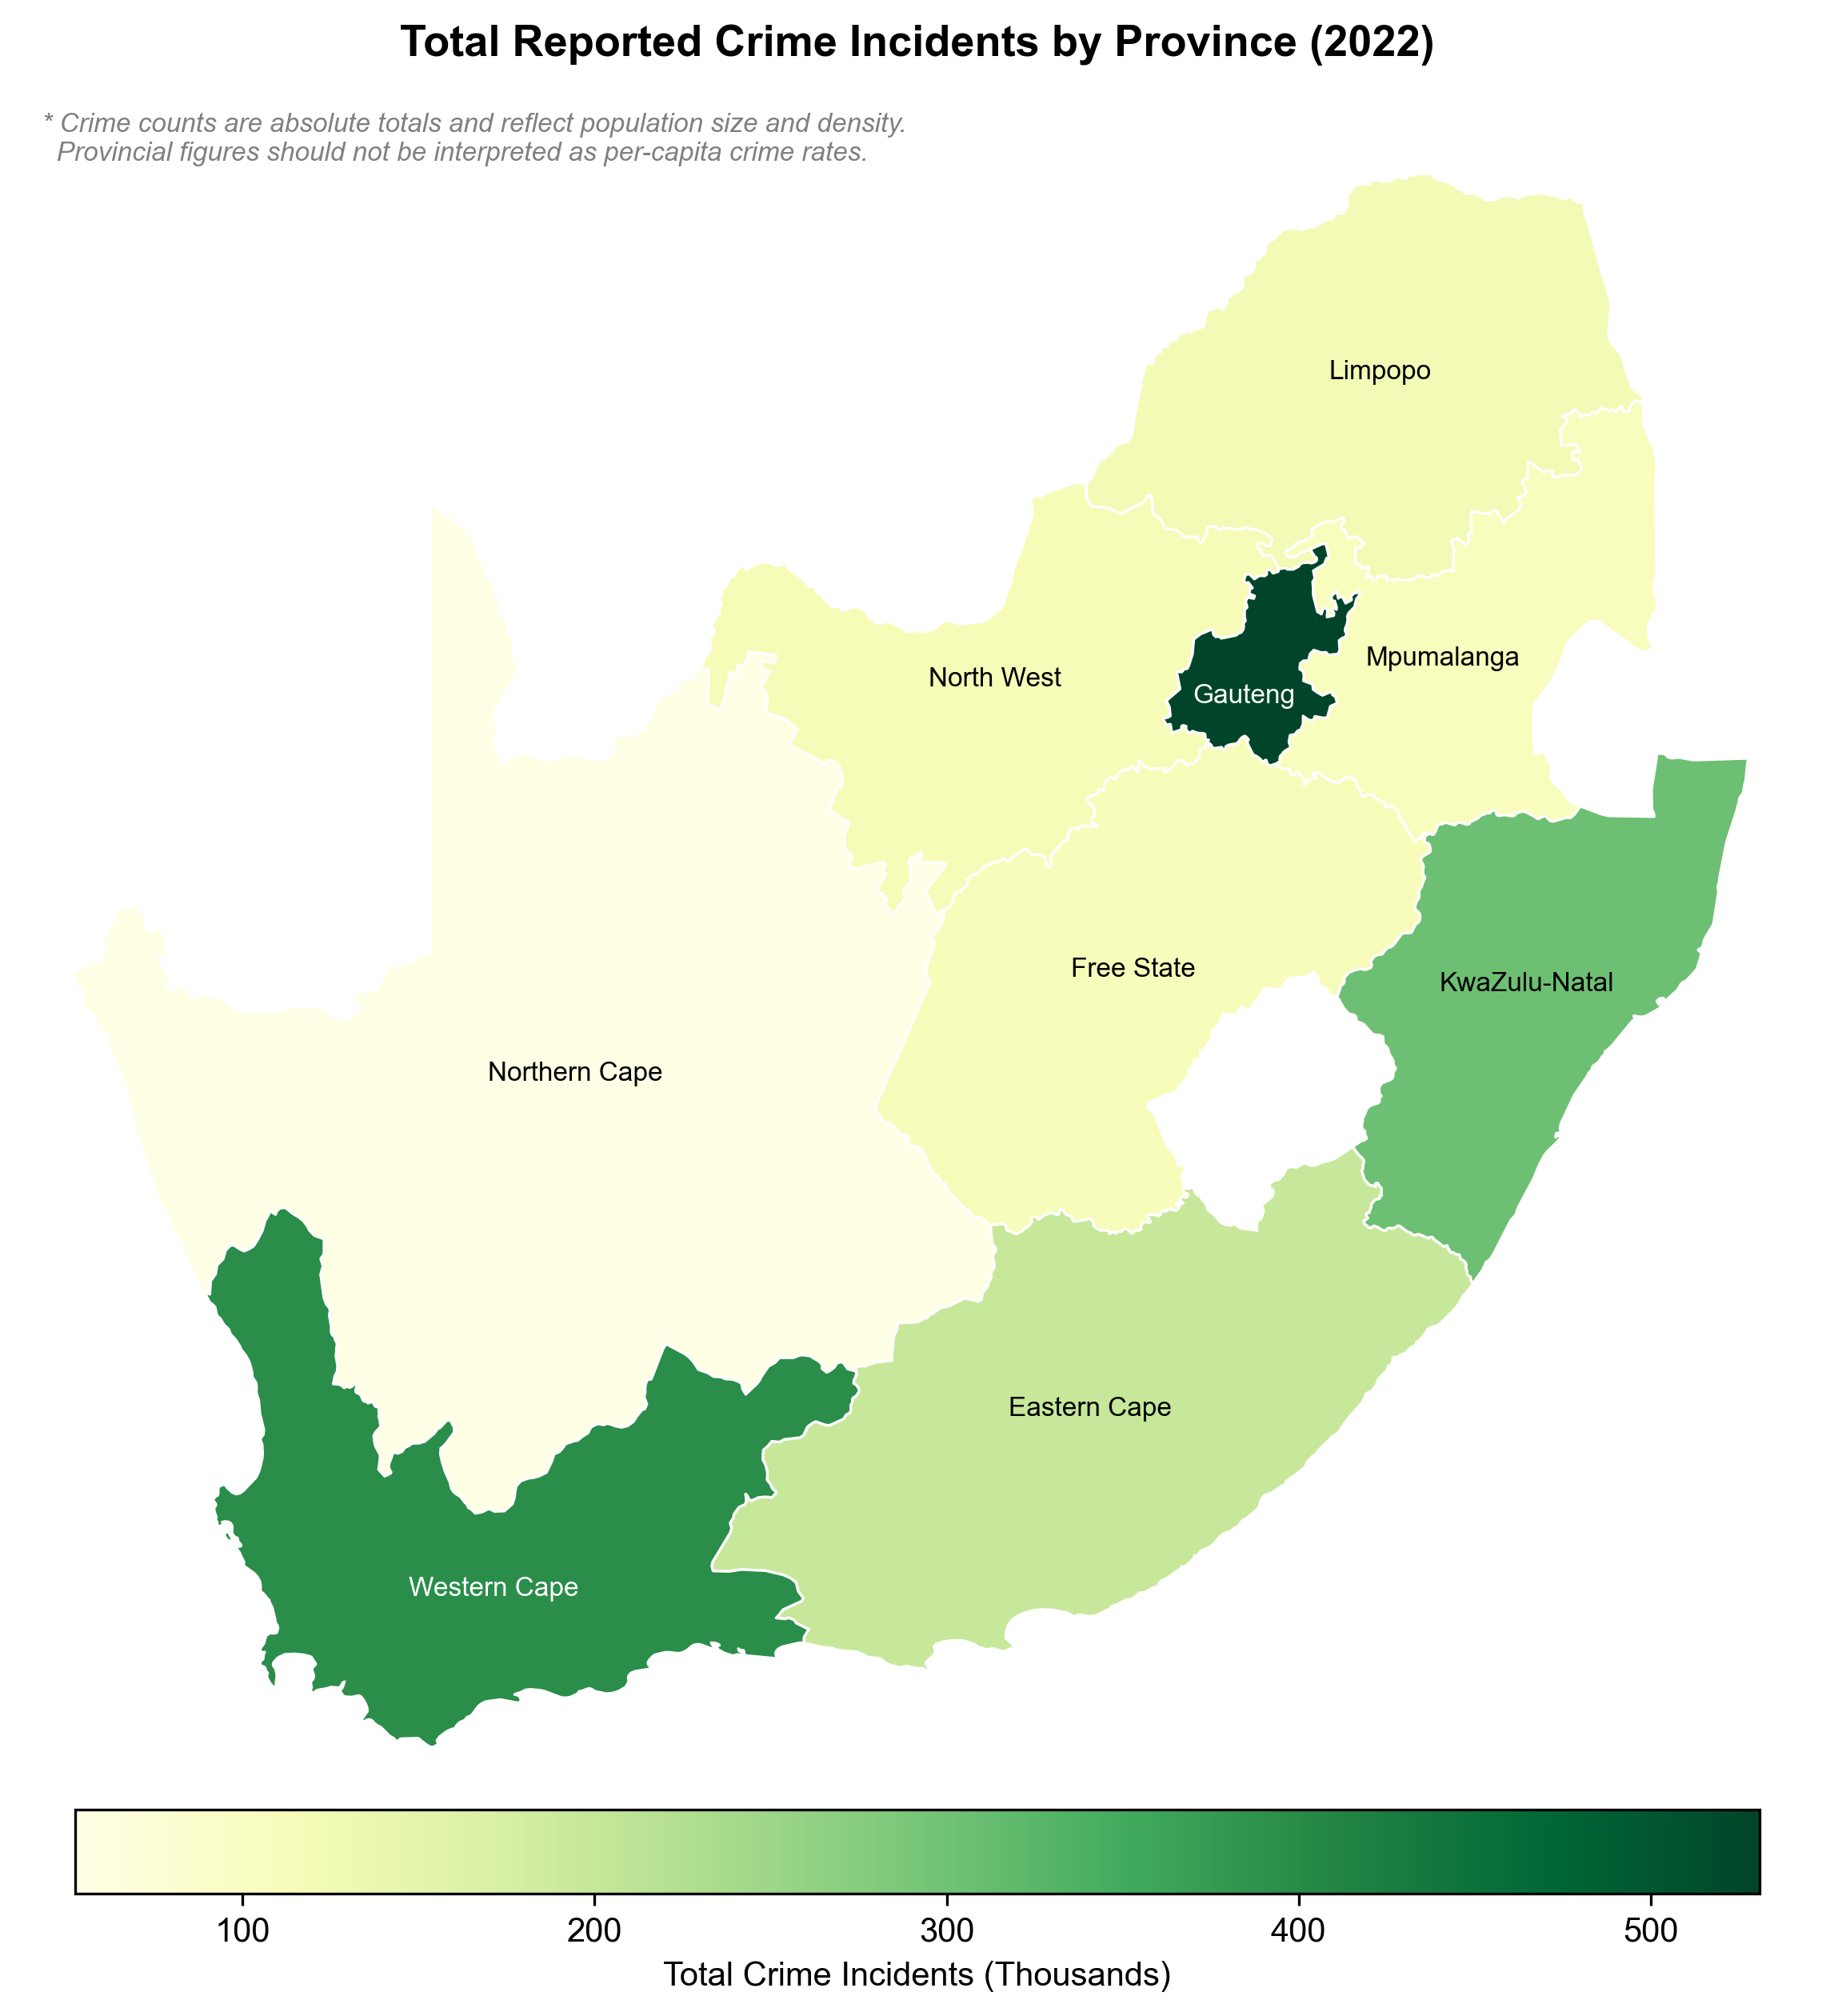
\includegraphics[width=\linewidth]{choropleth_2022.png}
		\caption{Choropleth map — total crime incidents by province, 2022 snapshot (Python — geopandas, matplotlib)}
		\label{fig:choropleth_2022}
	\end{figure}
	
	% ── SECTION 4 ─────────────────────────────────────────────────
	
	\newpage
	\section{MATLAB Trend Decomposition}
	
	\subsection{Moving Average Smoothing}
	
	% moving average equation placeholder:
	\begin{equation}
		\bar{x}_t = \frac{1}{3}\sum_{i=-1}^{1} x_{t+i}
		\label{eq:moving_average}
	\end{equation}
	
	\begin{figure}[H]
		\centering
		
		
\includegraphics[width=\linewidth]{trend_analysis.png}
		\caption{MATLAB — Contact crime trend decomposition: actual vs.\ 3-year moving average vs.\ linear trend (300 DPI)}
		\label{fig:trend_decomp}
	\end{figure}
	
	\subsection{Trend Interpretation}
	
	% ── SECTION 5 ─────────────────────────────────────────────────
	
	\newpage
	\section{Time Series Forecasting (RQ4)}
	
	\subsection{Model Selection}
	
	% ARIMA equation placeholder:
	\begin{equation}
		\phi(B)(1-B)^d X_t = \theta(B)\varepsilon_t
		\label{eq:arima}
	\end{equation}
	
	\subsection{COVID-19 Anomaly Handling}
	
	\subsection{Forecast Results}
	
	\begin{figure}[H]
		\centering
		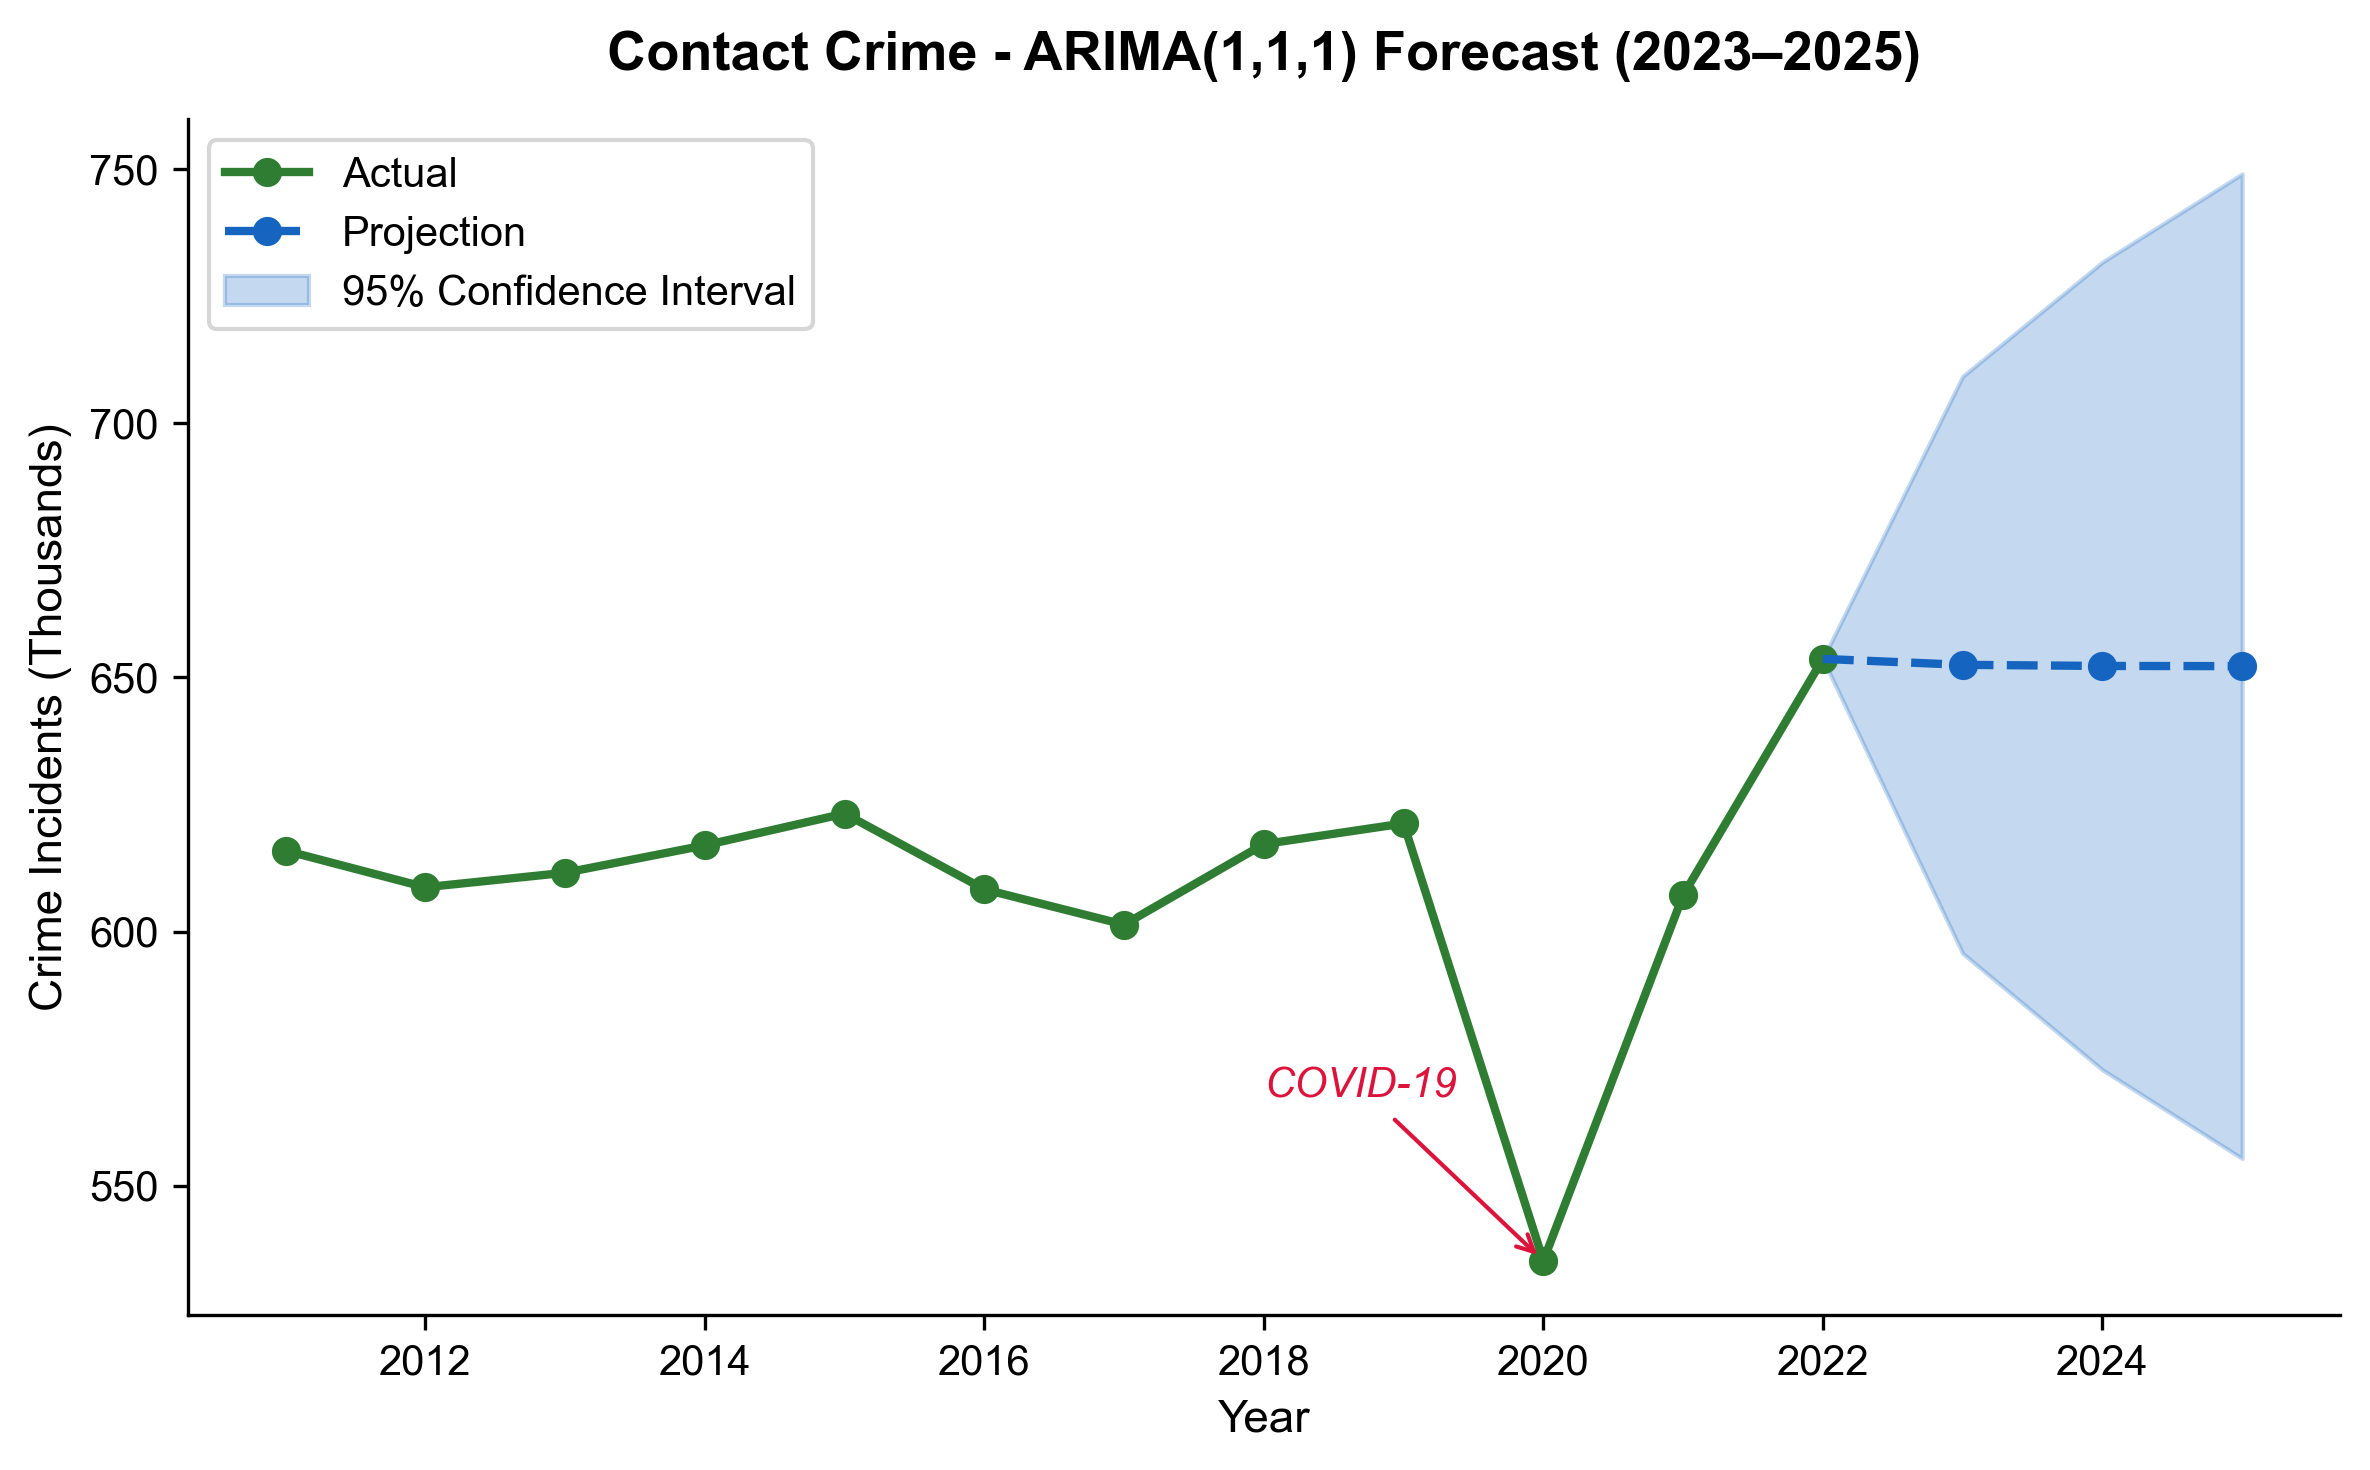
\includegraphics[width=\linewidth]{forecast_chart.png}
		\caption{ARIMA(1,1,1) 3-year forecast with 95\% confidence interval — Contact crime (Python — statsmodels)}
		\label{fig:forecast}
	\end{figure}
	
	% ── SECTION 6 ─────────────────────────────────────────────────
	
	\newpage
	\section{Key Findings}
	
	\begin{tcolorbox}[
		colback=green!5!white,
		colframe=green!60!black,
		title={\textbf{Key Findings}},
		fonttitle=\bfseries,
		rounded corners]
		\begin{itemize}
			\item \textbf{RQ1:} 
			\item \textbf{RQ2:} 
			\item \textbf{RQ3:} 
			\item \textbf{RQ4:} 
		\end{itemize}
	\end{tcolorbox}
	
	% ── SECTION 7 ─────────────────────────────────────────────────
	
	\newpage
	\section{Limitations}
	
	% ── SECTION 8 ─────────────────────────────────────────────────
	
	\newpage
	\section{Policy Implications}
	
	% ── SECTION 9 ─────────────────────────────────────────────────
	
	\newpage
	\section{Conclusion}
	
	% ── REFERENCES ────────────────────────────────────────────────
	
	\newpage
	\phantomsection
	\begin{thebibliography}{9}
		
		\bibitem{saps2023}
		South African Police Service. (2023). \textit{Annual Crime Report 2022/2023}. Pretoria: SAPS.
		
		\bibitem{kaggle}
		Agababyan, H. (2023). \textit{Crime Statistics of South Africa 2011--2023} [Dataset]. Kaggle. \url{https://www.kaggle.com/datasets/harutyunagababyan/crime-stats-of-south-africa-2011-2023}
		
		\bibitem{seabold2010}
		Seabold, S., \& Perktold, J. (2010). Statsmodels: Econometric and statistical modeling with Python. \textit{Proceedings of the 9th Python in Science Conference}.
		
		\bibitem{box2015}
		Box, G.E.P., Jenkins, G.M., Reinsel, G.C., \& Ljung, G.M. (2015). \textit{Time Series Analysis: Forecasting and Control} (5th ed.). Wiley.
		
		\bibitem{wickham2016}
		Wickham, H. (2016). \textit{ggplot2: Elegant Graphics for Data Analysis}. Springer.
		
		\bibitem{matlab}
		The MathWorks, Inc. (2024). \textit{MATLAB} (Version R2024a). \url{https://www.mathworks.com}
		
	\end{thebibliography}
	
	% ── APPENDICES ────────────────────────────────────────────────
	
	%\newpage
	%\appendix
	
	%\section{SQL Queries}
	%
	%\section{MATLAB Trend Decomposition Code}
	%
	%\section{R Cross-Validation}
	%
	%\subsection{Province Bar Chart}
	%
	%\begin{figure}[H]
	%	\centering
	%	\includegraphics[width=\linewidth]{r_province_bar.png}
	%	\caption{R — province bar chart, ggplot2 reproduction}
	%	\label{fig:r_province}
	%\end{figure}
	%
	%\subsection{National Crime Trend}
	%
	%\begin{figure}[H]
	%	\centering
	%	\includegraphics[width=\linewidth]{r_national_trend.png}
	%	\caption{R — national trend with geom\_smooth confidence band (ggplot2)}
	%	\label{fig:r_trend}
	%\end{figure}
	%
	%\subsection{Province Summary Statistics}
	
\end{document}